\section[Heat Capacity Models II — Einstein Revisited and Debye]{\hyperlink{toc}{Heat Capacity Models II — Einstein Revisited and Debye}}


\textbf{Einstein's model for specific heat}

\begin{itemize}
    \item Einsten improved upon Boltzmann's model by treating each atom as a quantum mechanical simple harmonic oscillator, still being held in place in each spatial direction by a spring that vibrates at a frequency, $\omega$.

    \[ E_n = \hbar \omega \paren*{n + \frac{1}{2}}\]

    where $\omega$ is the frequency of the spring, and n is the quantum number.

    \item Note that in this model the atoms are still not connected to each other.


    \item You can follow the steps:

    \begin{enumerate}
        \item Find $Z$
        \item $\avg{E} = \frac{-1}{Z} \dv{Z}{\beta},$
        \item $C = \dv{\avg{E}}{T}$
     \end{enumerate}

    and then you get 
    \[ C = 3R (\beta \hbar \omega)^2 \cdot \frac{\e^{\beta \hbar \omega}}{(\e^{\beta \hbar \omega} -1)^2}\]

    Note that this expression depends on temperature! 

    \item For HW1:

    \[ \sum_n x^n = \recip{1-x} \quad \text{for } \abs{x} < 1\]
    and
    \[ \sinh{(x)} = \frac{\e^x - \e^{-x}}{2}\]


    \item The \textbf{high T limit of Eistein's model} gives the expected \textbf{Dulong-Petit} value

    \[ \text{As} \quad T \rightarrow \infty, \, \beta \rightarrow 0  \]
    You can taylor expand for the exponential term in the denominator

    \[ C \approx 3R \cancel{(\beta \hbar \omega)^2} \cdot \frac{(1+ \cancelto{\sim 0}{\beta \hbar \omega})}{\cancel{(\beta \hbar \omega)^2}}\]

    \[ \boxed{C = 3R} \quad \text{which is the Dulong Petit value!}\]

    \item The \textbf{low T limit} accounts for the observation that specific heat decreases with T

    \[ \text{As} \qquad T \rightarrow 0, \, \beta \rightarrow \infty\]

    \[ C \approx 3R (\beta \hbar \omega)^2 \cdot \paren*{\frac{1}{\e^{\beta \hbar \omega}}}\]

    Correctly shows that 
    \[ \text{As } \quad T \rightarrow 0, \, C \rightarrow 0\]

    And also the discrepancy for diamond where C increased to 3R above room temp.

    But incorrectly suggests an exponential decrease at low T. The data (Einstein's 1907 paper) showed that at low T, $C \sim T^3$.

    \begin{center}
        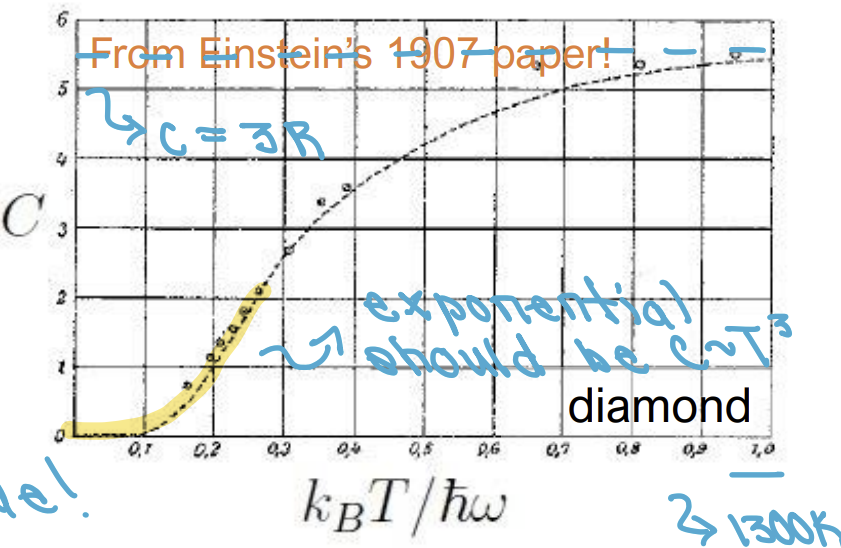
\includegraphics[width = 0.5\linewidth]{Images/einstein-1907.png}
    \end{center}

    \item Einstein temperature is then defined as 

    \[ T_E = \frac{\hbar \omega}{k_B}\]

    where you can think of a materials hardness to be related to the stiffness of the spring holding it in place

    \[ T_E \propto \omega , \quad \text{and} \quad \omega = \sqrt{\frac{k}{m}}\]

    so that the the mass of the atom also determines this temperature.

    \item You can calculate the typical frequency scale using a typical Einstein temperature using 
    \[ f = \frac{\omega}{2 \pi}\]

\end{itemize}

\textbf{Debye's model for specific heat}

\begin{itemize}
    \item Debye took Einstein's calculation one step further by realizing that \textbf{the atomic vibrations in solids are sound waves} and therefore -- not only should the energy levels be quantized -- but the energy should vary as a function of the wave vector, k.

    \begin{itemize}
        \item Einstein: $\omega=\text{constant}$
        \item Debye: $\omega(\vec{k}) = v \abs{\vec{k}}$
    \end{itemize}

    \item How should we think about the wavevector, k?

    e.g. 2D plane wave?

    \begin{center}
        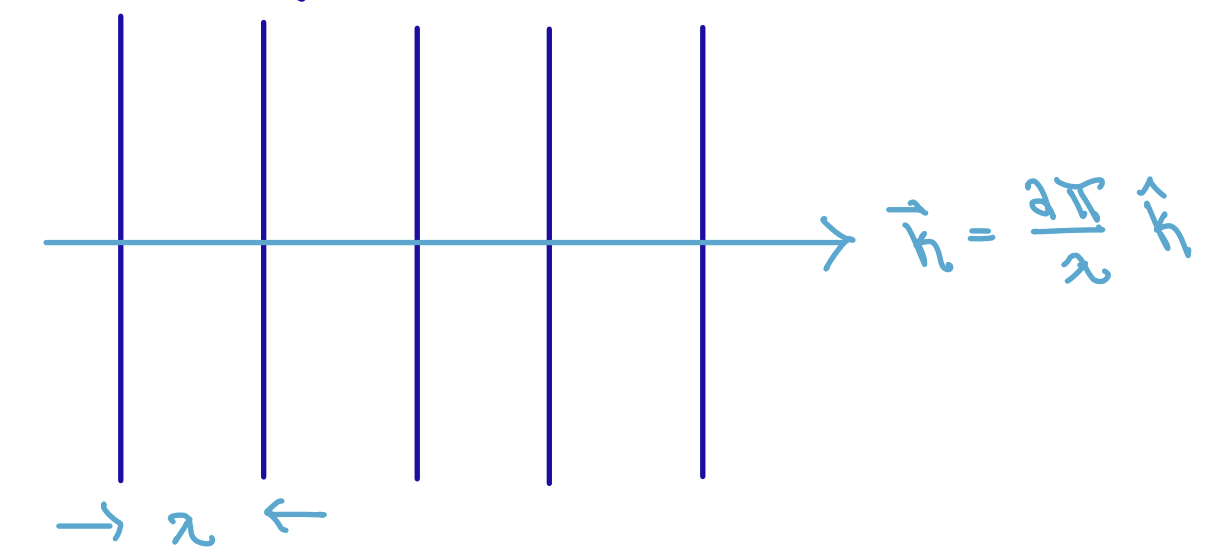
\includegraphics[width = 0.5 \linewidth]{Images/wavevector-k.png}
    \end{center}        

    k-space is useful because solids are periodic

    other names:

    \begin{itemize}
        \item momentum space 
        \item reciprocal space
        \item Q space
    \end{itemize}

    Normal space is called `` real space " 

\end{itemize}

\textbf{Periodic (Born-von Karman) boundary conditions}
(equivalet to particle in a box, but easier)
\begin{itemize}
    \item Rather than treating our solids as having fixed end points, it is very convenient to apply \textbf{periodic boundary conditions}. 
    
    \item In 1D this means taking a very long chain and attaching the ends together.
    \item Surfaces account for only a tiny fraction of a material so this is a reasonable thing to do.

    \begin{center}
        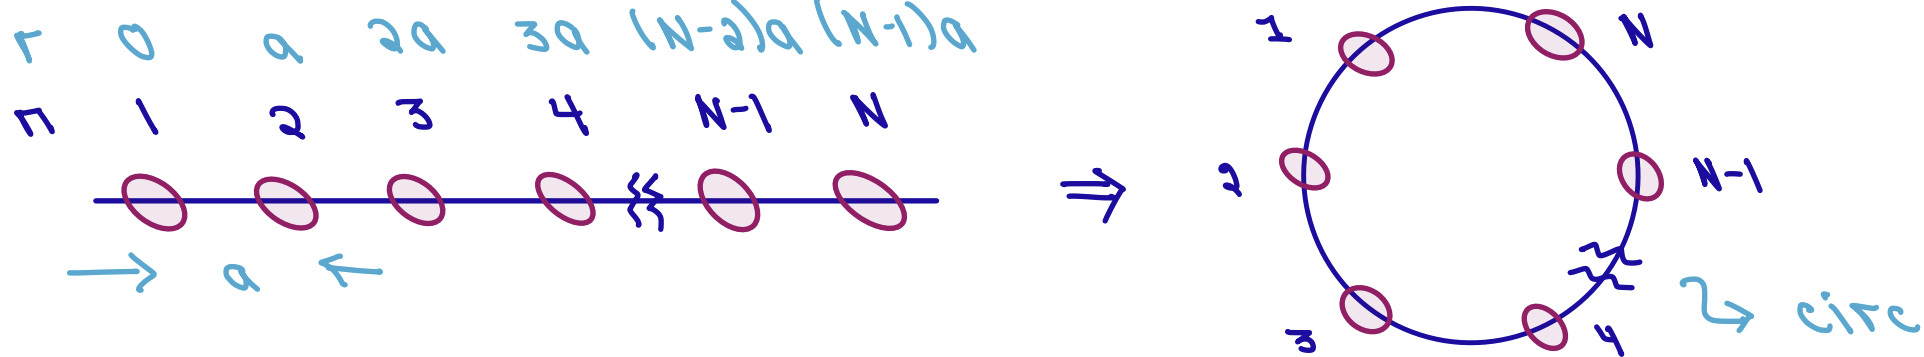
\includegraphics[width = 0.9 \linewidth]{Images/Born-von Karman - PBC.png}
    \end{center}

    \[ L = N \cdot a\]

    \item This imposes a condition on the possible k-values: the values of k are quantized!

    \item A wave $\e^{i k r}$ must have the same value at r and $r + L$:

    \[ \e^{i k r} = \e^{ik (r+L)} \Rightarrow \e^{i k L} = 1 \Rightarrow k \cdot L = 2 \pi n \quad (n=\text{integer}) \]

    \[ \boxed{k = \frac{2 \pi}{L} n}\]

    k is quantized! and $\Delta n = 1 \Rightarrow \boxed{\delta k = \frac{2\pi}{L}}$ so that $L \gg 1$, then $\delta k \ll 1$.

    \item In 3D ($v = L^3$) we can use the same trick excep the solid gets folded into a hypertorus.

    \begin{itemize}
        \item allowed k states $\quad \vec{k} = \frac{2\pi}{L} (n_x, n_y, n_z)$
        \item Volume of a k-point ($\Delta n_i = 1 : \quad \delta k = \paren*{\frac{2 \pi}{L}}^3$
    \end{itemize}

    \item Since the number of allowed wave vectors is discrete, we can count them:

        \[ \text{\#k-points} \, = \sum_k = \frac{\text{volume of k space}}{\text{volume of k point}} = \frac{\int d\vec{k}}{\paren*{\frac{2\pi}{L}}^3}\]

    \item We can convert the sum over all k to a 1D integral (assume spherical symmetry).

    \[ \int_{-\infty}^{\infty} \dd{\vb{k}} \rightarrow \int_{0}^{\infty} \dd{\phi} \int_{0}^{\pi} \dd{\theta} \sin{(\theta)} \cdot \int_{0}^{\infty} k^2 \dd{k}\]

    For the 3D. Can check 2D and 1D too.

    \item Now pulling the pieces together for Debye's model, we can calculate the specific heat by starting with an expression analogous to Einstein's except where $\omega$ depends on $\vb{k}$.

    \begin{itemize}
        \item Einstein:

        \[ \avg{E} = 3 \hbar \omega \brackets*{n_B (\beta \hbar \omega) + \frac{1}{2}}\]

        (from $\avg{E} = \frac{-1}{Z} \dv{Z}{\beta}$)
        \item Debye:
        \[ \avg{E} = 3 \sum_{\vb{k}} \hbar \omega(\vb{k})  \brackets*{n_B (\beta \hbar \omega(\vb{k})) + \frac{1}{2}}\]

        (where $\omega = v \abs{\vec{k}}$)
        
    \end{itemize}

    \item We can use the relationship above to then convert our sum to an integral --> Then, it is preferable to evaluate this integral with respect to $\omega$ instead of $k$.

    \begin{enumerate}
        \item Convert $\sum_{\vec{k}}$ to $\int 
        \dd{\vec{k}}$
        \item Convert 3D integral to 1D
        \item 3 Change of variable , $k=\frac{\omega}{v}$, $\dd{k} = \frac{1}{v} \dd{\omega}$
        \item Result: 

        \[ \avg{E} = \int_0^{\infty} \dd{\omega} \cdot \brackets*{L^3 \cdot \frac{12 \pi \omega^2}{(2 \pi)^3 v^3 }} \hbar \omega \paren*{n_B(\beta \hbar \omega) + \frac{1}{2}}\]

        Note the velocity term!
    \end{enumerate}
    
\end{itemize}



